\documentclass[10pt]{article}

% ----- Packages -----
\usepackage[paperwidth=7.5in, paperheight=10.3in, top=1in, bottom=1in, left=0.6in, right=0.6in]{geometry}
\usepackage{titlesec}
\usepackage{graphicx}
\usepackage{caption}
\usepackage{amsmath}
\usepackage{enumitem}
\usepackage{fancyhdr}
\usepackage{mathpazo}  % Substitute for Lucida Bright
\usepackage{hyperref}
\usepackage{wrapfig}
\usepackage{pdfpages}
\usepackage{graphicx} % You already have this



% ----- Hyphenation -----
\hyphenation{Zep-CAD Zeppelin}

% ----- Header/Footer -----
\pagestyle{fancy}
\fancyhf{}
\lhead{Computer-Aided Design \& Applications, \today}
\rfoot{\thepage}
\renewcommand{\headrulewidth}{0pt}

% ----- Section Formatting -----
\titleformat{\section}{\bfseries\uppercase}{\thesection}{1em}{}
\titleformat{\subsection}{\bfseries}{\thesubsection}{1em}{}

% ----- Title -----
\title{\bfseries Zep-CAD: MINI-CAD SOFTWARE FOR ZEPPELIN MODELING}
\author{
    Evan Blosser (34\%)$^{1}$, \\
    Matthew Dobbs (33\%)$^{1}$, \\
    Blake T Johnson (33\%)$^{1}$,  \\
{\small $^{1}$University of Oklahoma, evan.a.blosser-1@ou.edu} \\
{\small $^{1}$University of Oklahoma, mdobbs@ou.edu} \\
{\small $^{1}$University of Oklahoma, blake.t.ohnson-1@ou.edu} \\
}
\date{\today}

\begin{document}

%\begin{center}
    %\includegraphics[width=1in]{logo.png} \\[0.2em]
%\end{center}


\maketitle


\vspace{-1em}
\noindent\rule{\textwidth}{0.4pt}

% ----------- Abstract -----------

\begin{center}
    \textbf{ABSTRACT}
\end{center}
{\small
This paper presents \textbf{Zep-CAD}, a mini-CAD software developed in Python for the parametric design and 3D 
visualization of rigid-body Zeppelin airships. Zep-CAD enables users to define the shape and configuration of 
four main components—envelope, gondola, engines, and fins—using industry-standard modeling techniques such as 
cubic splines, Bézier and B-spline curves, lofted and ruled surfaces, and revolved geometry. The software 
features a tab-based graphical user interface built with PySide6, providing real-time updates as users modify 
geometric parameters. Surface generation is driven by symbolic and numerical computation using SymPy and NumPy, 
with visualization handled by Matplotlib. Zep-CAD is designed to support rapid design iteration, clear component 
modularity, and geometric precision, making it suitable for conceptual airship modeling. While advanced features 
such as solid rendering and STL export are under development, Zep-CAD provides a robust foundation for educational 
and exploratory CAD workflows.
}

    

\vspace{1em}
\noindent
\textbf{Keywords:} zeppelin design, CAD software, B-spline, Bezier curves, parametric modeling

\vspace{0.5em}
\noindent
\textbf{DOI:} 04-29-2025



% ----------- MAIN SECTIONS -----------
\section{INTRODUCTION}

The goal of this project is to develop \textbf{Zep-CAD}, a custom-built computer-aided design (CAD) software 
written in Python that enables users to create and visualize parametric models of rigid-body Zeppelin airships. 
Inspired by classic and speculative airship designs, the software facilitates early-stage conceptual design by 
allowing users to adjust geometric parameters interactively and observe the effects on envelope shape, gondola 
size and position, engine pod placement, and fin configuration.

Zep-CAD supports multiple curve and surface types used in industry-standard modeling workflows. These include 
cubic splines for the main envelope profile, Bézier and lofted surfaces for the gondola, quadratic splines with 
ruled surfaces for the stabilizing fins, and B-splines combined with revolved surfaces for engine pods. Each 
geometric element is defined parametrically and plotted in 3D space using real-time graphical feedback. This 
approach allows designers to evaluate aesthetics and proportion before proceeding to detailed structural or 
aerodynamic analysis.

The project emphasizes clarity of modeling technique, full parametric control, and accessibility of the tool. 
Zep-CAD is built with PySide6 for its graphical user interface, SymPy and NumPy for symbolic and numerical 
computations, and Matplotlib for 3D visualization. A tab-based UI structure separates design modules (Envelope, 
Gondola, Engine, and Fins), ensuring an intuitive workflow while supporting successive redraws and configuration 
variations.

This report documents the architecture, implementation, capabilities, and limitations of Zep-CAD. It also 
reflects on the development process and provides a technical self-assessment in accordance with course 
expectations. All plots, figures, and sample models are included in Appendix A.



\section{SOFTWARE ARCHITECTURE}

Zep-CAD is a modular Python application designed to provide an intuitive interface for early-stage airship design. 
The software features a tab-based graphical user interface (GUI) developed with PySide6 and a backend structure 
organized into independent geometry modules. Each component of the Zeppelin—envelope, gondola, engines, and 
fins—is generated based on user-defined parameters, providing real-time updates in a 3D wireframe view.

The GUI layout is divided into two primary regions: a left-side control panel containing input tabs, and a 
right-side 3D visualization window powered by Matplotlib. Users select design parameters such as dimensions, 
positions, and quantities via text fields and sliders. Upon pressing the draw buttons, the associated surfaces 
are constructed and plotted interactively. The GUI also includes functionality to clear the plot, reset views, 
and save images. The GUI layout and modular architecture are based on standard CAD/CAE design 
practices~\cite{chang2014}, promoting independent development of each component and flexible parameter control.


Internally, the application is modularized into separate Python scripts, each responsible for generating a 
specific component:
\begin{table}[h!]
    \centering
    \caption{Zep-CAD Component Curve and Surface Summary}
    \begin{tabular}{|l|l|l|}
    \hline
    \textbf{Component} & \textbf{Curve Type} & \textbf{Surface Type} \\
    \hline
    Envelope & Cubic spline & Revolved surface \\
    Gondola & Quadratic Bézier curves & Lofted + Revolved caps \\
    Engine & Quadratic B-spline & Revolved surface + Translation \\
    Fins & Quadratic spline & Ruled surface + Rotation \\
    \hline
    \end{tabular}
\end{table}


Control logic is handled through \texttt{main.py}, which connects GUI inputs to surface generation functions and manages real-time plot updates. SymPy and NumPy libraries are used for symbolic equation generation and numerical evaluation, respectively. All surfaces are displayed as wireframe models to optimize responsiveness during design iteration.

\begin{figure}[h!]
    \centering
    \begin{minipage}{0.45\textwidth}
        \centering
        \includegraphics[width=\textwidth]{gui_layout.png} % (GUI layout screenshot)
        \caption{Zep-CAD GUI Layout.}
    \end{minipage}%
    \hfill
    \begin{minipage}{0.45\textwidth}
        \centering
        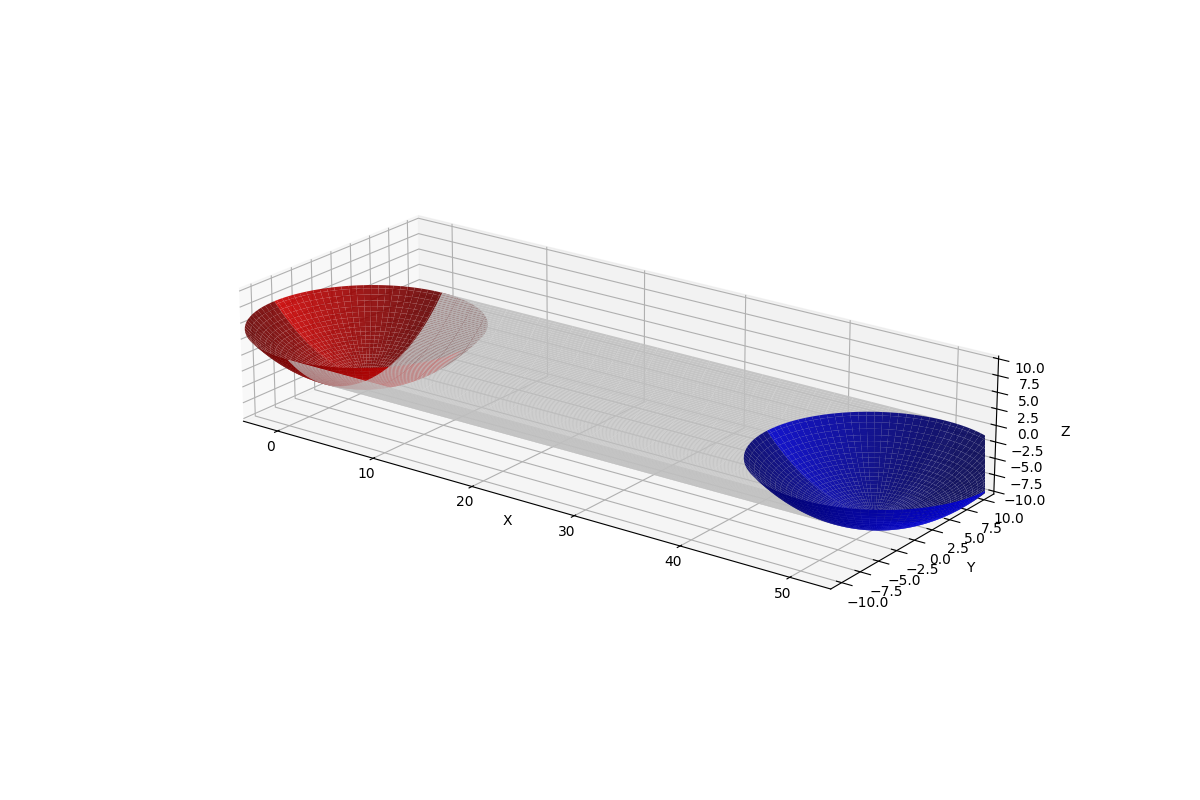
\includegraphics[width=\textwidth]{gondola1.png} % (Gondola example screenshot)
        \caption{Gondola Geometry Example.}
    \end{minipage}
\end{figure}





\section{GEOMETRIC MODELING IMPLEMENTATION}

Zep-CAD supports a range of parametric curves and surface generation techniques, enabling users to construct an 
idealized rigid-body Zeppelin model. Standard modeling techniques such as Bézier and B-spline curves are applied 
following common CAD/CAE design principles~\cite{farin2002, piegl1997}. Each component is created using symbolic
equations evaluated numerically over user-defined parameter ranges. This section outlines the mathematical 
formulation and CAD techniques applied to each of the four modeled elements.

\subsection{Envelope: Cubic Spline with Revolved Surface}

The main body of the Zeppelin is generated from a four-point cubic spline defined in the x–z plane. Users 
provide the overall length of the envelope, the maximum radius, and the position of the control points along the 
length to control nose sharpness. These control points define the profile curve, which is then revolved 360 
degrees about the x-axis to produce a closed, axisymmetric surface. The revolution is implemented through 
parametric equations evaluated with meshgrids over \( u \in [0, 1] \) and \( \theta \in [0, 2\pi] \).
\begin{figure}[h!]
    \centering
    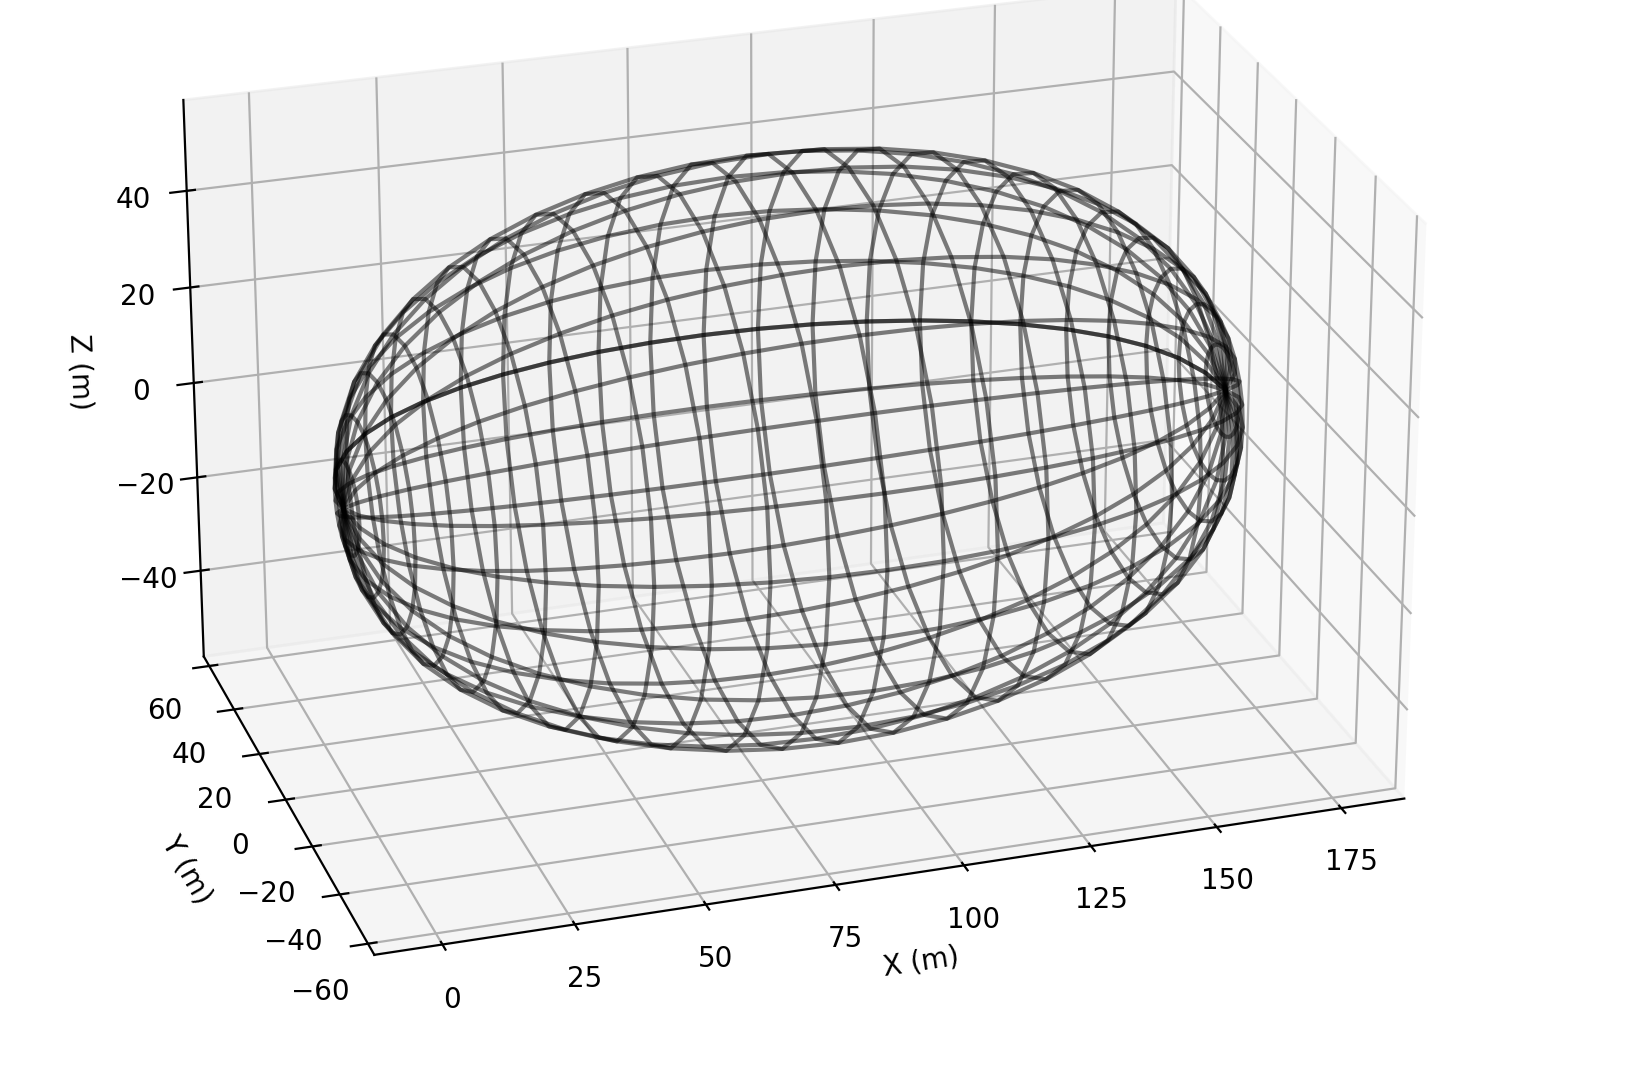
\includegraphics[width=0.5\textwidth]{envelope_profile.png} % placeholder name
    \caption{Example Envelope Profile generated by Cubic Spline and Revolution.}
\end{figure}


\subsection{Gondola: Quadratic Bézier Lofted Surface with Revolved Caps}

The gondola is constructed using a pair of quadratic Bézier curves to define the front and rear cross-sections. 
These curves are lofted together along the x-direction to form the main body of the gondola. To complete the 
shape, revolved surfaces are generated from the Bézier control profiles at both ends, using a semi-circular 
sweep (\( \theta \in [0, \pi] \)). The entire structure is then translated in 3D space to align with the lowest 
point of the envelope based on its computed bounding box.
\par
Where the gondola body meets the envelope, intersection curves naturally form between the lofted gondola surface 
and the revolved envelope surface. While the current implementation focuses on maintaining a smooth alignment 
visually, future work will incorporate using these intersection lines to trim the gondola geometry precisely to 
the envelope, ensuring a clean and snug fit.

\begin{figure}[h!]
    \centering
    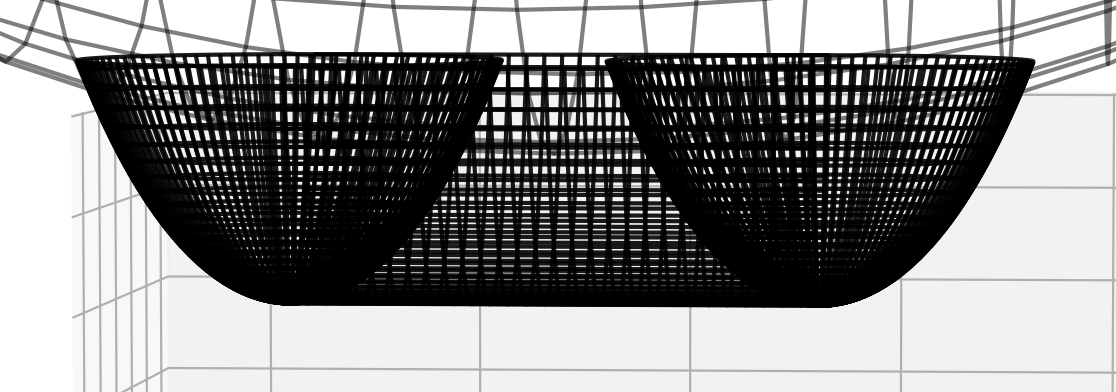
\includegraphics[width=0.5\textwidth]{gondola_surface.png} % placeholder name
    \caption{Lofted Gondola Surface with Revolved End Caps.}
\end{figure}



\subsection{Fins: Quadratic Spline with Ruled and Mirrored Surfaces}

Each fin is defined by a quadratic spline based on three control points forming the airfoil shape. A ruled 
surface is constructed between the base airfoil and a scaled, offset version at the tip. An identical mirrored 
surface is generated by reflecting the airfoil geometry about the xz-plane. The complete fin is thus formed from 
two ruled patches. The user specifies the number of fins, which are then distributed evenly around the envelope 
by applying a rotation matrix about the x-axis.

\begin{figure}[h!]
    \centering
    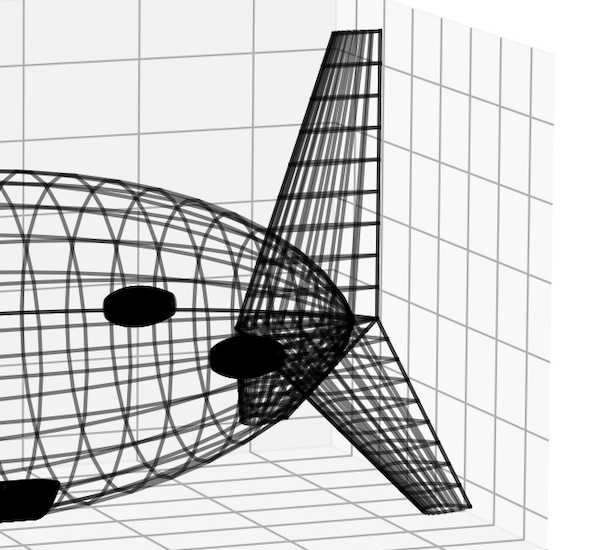
\includegraphics[width=0.5\textwidth]{fin_1.png} % placeholder name
    \caption{Ruled Surface Fins arranged around the Envelope.}
\end{figure}


\subsection{Engine: B-Spline Profile with Revolved Surface and Translation}

The engine nacelle is defined using a four-point quadratic B-spline curve in the x–z plane. This curve controls 
the pod’s profile, which is revolved about the x-axis to form a symmetric surface. The final geometry is 
translated laterally from the main body using a homogeneous transformation matrix. The user specifies pod 
length, radius, taper, and axial position along the envelope as input parameters.



\section{CAPABILITIES AND LIMITATIONS}

\subsection{Supported Curves and Surfaces}

Zep-CAD implements four curve types and three primary surface generation methods to construct Zeppelin components.
 Cubic splines are used for the envelope profiles, quadratic Bézier curves shape the gondola sections, quadratic 
 splines define the fins, and B-splines create engine pods. Surface generation techniques include revolved 
 surfaces (for the envelope, engine pods, and gondola end caps), lofted surfaces (for the gondola body), and 
 ruled surfaces (for the fins). Geometric transformations such as translation and rotation are applied to 
 accurately position gondolas, engines, and fins. A full summary is provided in Appendix A, Table 1.


\subsection{Software Capabilities}

Zep-CAD allows users to dynamically modify all geometric parameters and regenerate the corresponding surfaces in 
real time. Each component is modeled independently, enabling isolated design iterations. The GUI supports 
multiple redraws, visual feedback through a wireframe 3D plot, and basic layout validation (e.g., fin count,
 engine position limits). Surface generation is done symbolically and numerically, supporting precise 
 definitions and scalability.

 \subsection{Current Limitations}

 While Zep-CAD achieves its core modeling objectives, several simplifications are present. Surfaces are 
 displayed in wireframe format only, with no solid rendering or STL export. Gondola positioning is restricted to
  the bottom centerline of the envelope, and only a single gondola is supported per model. Engines and fins are 
  limited to axis-aligned placements without skewed orientations. No simulation, structural analysis, or 
  manufacturability checking tools are integrated. These constraints were accepted to prioritize software 
  clarity, responsiveness, and focus on parametric surface generation.
 

  \section{LESSONS LEARNED}

  Developing Zep-CAD provided valuable insights into both CAD theory and practical Python implementation. A key 
  technical challenge was handling symbolic expressions for curve and surface generation, requiring careful use 
  of SymPy and NumPy to ensure performance and accuracy. The project reinforced the importance of spatial 
  reasoning, particularly in applying Bézier and B-spline formulations, parametric equations, and geometric 
  transformations like translation and rotation.
  
  Modular code architecture and GUI development using PySide6 highlighted the importance of separating interface 
  logic from computation, improving code clarity and maintainability. Finally, effective collaboration and scope 
  management were critical to delivering a complete tool within time constraints, requiring efficient iteration, 
  testing, and adaptation to evolving project needs.
  

  \section{SELF-ASSESSMENT}

  Zep-CAD provides a flexible platform for parametric design iteration and has been successfully tested across a 
  variety of realistic and stylized Zeppelin configurations. Future development will focus on expanding 
  functionality, including enhancements such as STL export capabilities and refined surface-to-surface 
  intersection handling to improve model integration. Based on the achieved functionality, usability, and 
  adherence to project goals, Zep-CAD is considered a complete and successful mini-CAD software for airship 
  modeling.
  


\newpage

% ----------- REFERENCES -----------
\bibliographystyle{plain}
\bibliography{references}

\newpage


\appendix
\section*{APPENDIX A: SUPPLEMENTAL MATERIALS}
\addcontentsline{toc}{section}{Appendix A: Supplemental Materials}

\subsection*{Table 1: Curve, Surface, and Transformation Summary}

\begin{center}
\begin{tabular}{|l|l|l|l|}
\hline
\textbf{Component} & \textbf{Curve Type} & \textbf{Surface Type} & \textbf{Transformation} \\
\hline
Envelope & Cubic spline (4-pt) & Revolved surface & None \\
Gondola & Bézier curve (5-pt) & Lofted + Revolved caps & Translation (to envelope base) \\
Fins & Quadratic spline (3-pt) & Ruled surface (top/bottom) & Rotation (radial spacing) \\
Engine & B-spline (4-pt) & Revolved surface & Translation (offset position) \\
\hline
\end{tabular}
\end{center}

\vspace{1em}

\subsection*{Supplemental Figures}

\begin{itemize}
    \item \textbf{Figure A1:} Zep-CAD Main GUI Layout
    \item \textbf{Figure A2:} Example Envelope Profile (Cubic Spline and Revolution)
    \item \textbf{Figure A3:} Gondola Lofted Surface with Revolved End Caps
    \item \textbf{Figure A4:} Fin Geometry using Ruled Surfaces
    \item \textbf{Figure A5:} Full Zeppelin Model Example
\end{itemize}

\vspace{1em}

\subsection*{Design Change Example: Modified Envelope}

We ran several tests and designs to in order to test and demonstrate the systems capabilities. Included below are 
a few examples of the tests that we ran. These examples follow parametric design adjustment strategies commonly 
applied in early-stage CAD modeling workflows~\cite{chang2014}.


To demonstrate flexible design iteration, the envelope profile was adjusted by modifying the location of the 
first control point, resulting in a sharper nose cone configuration. This change was applied in real time 
through the GUI and regenerated the revolved envelope surface immediately.

\begin{figure}[h!]
    \centering
    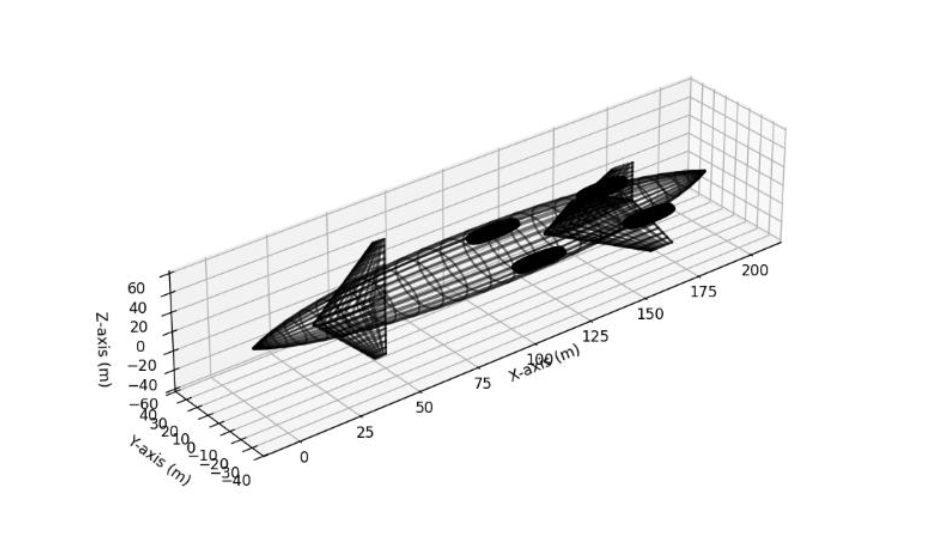
\includegraphics[width=0.6\textwidth]{dart.png} % Replace with actual filename
    \caption{Modified Envelope Profile showing Sharper Nose through Control Point Adjustment.}
\end{figure}

%Additionally we tested the design with single fins and smaller gondolas, as shown in the figure below.
%\begin{figure}[h!]
    %\centering
    %\includegraphics[width=0.6\textwidth]{single_fin.png} % Replace with actual filename
    %\caption{Example of a Zeppelin Model with Single Fin and Smaller Gondola.}
%\end{figure}

We also tested a wider envelope configuration by increasing the maximum radius, as shown in the figure below.

\begin{figure}[h!]
    \centering
    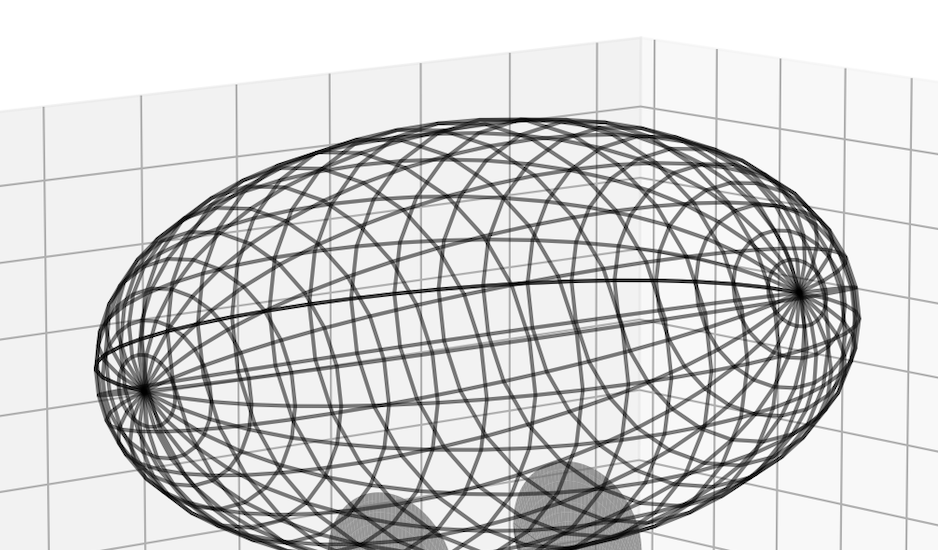
\includegraphics[width=0.6\textwidth]{wide.png} % Replace with actual filename
    \caption{Example of a Zeppelin Model with Wider Envelope and Larger Radius.}
\end{figure}

Additional test models, including variations in gondola size, fin configurations, and engine placements, were 
developed and are provided in the User Guide. 

\subsection*{User Manual}

A complete user manual is included in the submission folder as \texttt{Zep-CAD\_User\_Guide.pdf}
, covering:
\begin{itemize}
    \item UI input descriptions
    \item Step-by-step build instructions
    \item Troubleshooting notes
\end{itemize}



\end{document}

